% Generated by Sphinx.
\def\sphinxdocclass{report}
\documentclass[letterpaper,10pt,english]{sphinxmanual}
\usepackage[utf8]{inputenc}
\DeclareUnicodeCharacter{00A0}{\nobreakspace}
\usepackage{cmap}
\usepackage[T1]{fontenc}
\usepackage{babel}
\usepackage{times}
\usepackage[Bjarne]{fncychap}
\usepackage{longtable}
\usepackage{sphinx}
\usepackage{multirow}


\title{Science2Fiction}
\date{November 26, 2014}
\release{3.14}
\author{OctoMiao}
\newcommand{\sphinxlogo}{}
\renewcommand{\releasename}{Release}
\makeindex

\makeatletter
\def\PYG@reset{\let\PYG@it=\relax \let\PYG@bf=\relax%
    \let\PYG@ul=\relax \let\PYG@tc=\relax%
    \let\PYG@bc=\relax \let\PYG@ff=\relax}
\def\PYG@tok#1{\csname PYG@tok@#1\endcsname}
\def\PYG@toks#1+{\ifx\relax#1\empty\else%
    \PYG@tok{#1}\expandafter\PYG@toks\fi}
\def\PYG@do#1{\PYG@bc{\PYG@tc{\PYG@ul{%
    \PYG@it{\PYG@bf{\PYG@ff{#1}}}}}}}
\def\PYG#1#2{\PYG@reset\PYG@toks#1+\relax+\PYG@do{#2}}

\expandafter\def\csname PYG@tok@gd\endcsname{\def\PYG@tc##1{\textcolor[rgb]{0.63,0.00,0.00}{##1}}}
\expandafter\def\csname PYG@tok@gu\endcsname{\let\PYG@bf=\textbf\def\PYG@tc##1{\textcolor[rgb]{0.50,0.00,0.50}{##1}}}
\expandafter\def\csname PYG@tok@gt\endcsname{\def\PYG@tc##1{\textcolor[rgb]{0.00,0.27,0.87}{##1}}}
\expandafter\def\csname PYG@tok@gs\endcsname{\let\PYG@bf=\textbf}
\expandafter\def\csname PYG@tok@gr\endcsname{\def\PYG@tc##1{\textcolor[rgb]{1.00,0.00,0.00}{##1}}}
\expandafter\def\csname PYG@tok@cm\endcsname{\let\PYG@it=\textit\def\PYG@tc##1{\textcolor[rgb]{0.25,0.50,0.56}{##1}}}
\expandafter\def\csname PYG@tok@vg\endcsname{\def\PYG@tc##1{\textcolor[rgb]{0.73,0.38,0.84}{##1}}}
\expandafter\def\csname PYG@tok@m\endcsname{\def\PYG@tc##1{\textcolor[rgb]{0.13,0.50,0.31}{##1}}}
\expandafter\def\csname PYG@tok@mh\endcsname{\def\PYG@tc##1{\textcolor[rgb]{0.13,0.50,0.31}{##1}}}
\expandafter\def\csname PYG@tok@cs\endcsname{\def\PYG@tc##1{\textcolor[rgb]{0.25,0.50,0.56}{##1}}\def\PYG@bc##1{\setlength{\fboxsep}{0pt}\colorbox[rgb]{1.00,0.94,0.94}{\strut ##1}}}
\expandafter\def\csname PYG@tok@ge\endcsname{\let\PYG@it=\textit}
\expandafter\def\csname PYG@tok@vc\endcsname{\def\PYG@tc##1{\textcolor[rgb]{0.73,0.38,0.84}{##1}}}
\expandafter\def\csname PYG@tok@il\endcsname{\def\PYG@tc##1{\textcolor[rgb]{0.13,0.50,0.31}{##1}}}
\expandafter\def\csname PYG@tok@go\endcsname{\def\PYG@tc##1{\textcolor[rgb]{0.20,0.20,0.20}{##1}}}
\expandafter\def\csname PYG@tok@cp\endcsname{\def\PYG@tc##1{\textcolor[rgb]{0.00,0.44,0.13}{##1}}}
\expandafter\def\csname PYG@tok@gi\endcsname{\def\PYG@tc##1{\textcolor[rgb]{0.00,0.63,0.00}{##1}}}
\expandafter\def\csname PYG@tok@gh\endcsname{\let\PYG@bf=\textbf\def\PYG@tc##1{\textcolor[rgb]{0.00,0.00,0.50}{##1}}}
\expandafter\def\csname PYG@tok@ni\endcsname{\let\PYG@bf=\textbf\def\PYG@tc##1{\textcolor[rgb]{0.84,0.33,0.22}{##1}}}
\expandafter\def\csname PYG@tok@nl\endcsname{\let\PYG@bf=\textbf\def\PYG@tc##1{\textcolor[rgb]{0.00,0.13,0.44}{##1}}}
\expandafter\def\csname PYG@tok@nn\endcsname{\let\PYG@bf=\textbf\def\PYG@tc##1{\textcolor[rgb]{0.05,0.52,0.71}{##1}}}
\expandafter\def\csname PYG@tok@no\endcsname{\def\PYG@tc##1{\textcolor[rgb]{0.38,0.68,0.84}{##1}}}
\expandafter\def\csname PYG@tok@na\endcsname{\def\PYG@tc##1{\textcolor[rgb]{0.25,0.44,0.63}{##1}}}
\expandafter\def\csname PYG@tok@nb\endcsname{\def\PYG@tc##1{\textcolor[rgb]{0.00,0.44,0.13}{##1}}}
\expandafter\def\csname PYG@tok@nc\endcsname{\let\PYG@bf=\textbf\def\PYG@tc##1{\textcolor[rgb]{0.05,0.52,0.71}{##1}}}
\expandafter\def\csname PYG@tok@nd\endcsname{\let\PYG@bf=\textbf\def\PYG@tc##1{\textcolor[rgb]{0.33,0.33,0.33}{##1}}}
\expandafter\def\csname PYG@tok@ne\endcsname{\def\PYG@tc##1{\textcolor[rgb]{0.00,0.44,0.13}{##1}}}
\expandafter\def\csname PYG@tok@nf\endcsname{\def\PYG@tc##1{\textcolor[rgb]{0.02,0.16,0.49}{##1}}}
\expandafter\def\csname PYG@tok@si\endcsname{\let\PYG@it=\textit\def\PYG@tc##1{\textcolor[rgb]{0.44,0.63,0.82}{##1}}}
\expandafter\def\csname PYG@tok@s2\endcsname{\def\PYG@tc##1{\textcolor[rgb]{0.25,0.44,0.63}{##1}}}
\expandafter\def\csname PYG@tok@vi\endcsname{\def\PYG@tc##1{\textcolor[rgb]{0.73,0.38,0.84}{##1}}}
\expandafter\def\csname PYG@tok@nt\endcsname{\let\PYG@bf=\textbf\def\PYG@tc##1{\textcolor[rgb]{0.02,0.16,0.45}{##1}}}
\expandafter\def\csname PYG@tok@nv\endcsname{\def\PYG@tc##1{\textcolor[rgb]{0.73,0.38,0.84}{##1}}}
\expandafter\def\csname PYG@tok@s1\endcsname{\def\PYG@tc##1{\textcolor[rgb]{0.25,0.44,0.63}{##1}}}
\expandafter\def\csname PYG@tok@gp\endcsname{\let\PYG@bf=\textbf\def\PYG@tc##1{\textcolor[rgb]{0.78,0.36,0.04}{##1}}}
\expandafter\def\csname PYG@tok@sh\endcsname{\def\PYG@tc##1{\textcolor[rgb]{0.25,0.44,0.63}{##1}}}
\expandafter\def\csname PYG@tok@ow\endcsname{\let\PYG@bf=\textbf\def\PYG@tc##1{\textcolor[rgb]{0.00,0.44,0.13}{##1}}}
\expandafter\def\csname PYG@tok@sx\endcsname{\def\PYG@tc##1{\textcolor[rgb]{0.78,0.36,0.04}{##1}}}
\expandafter\def\csname PYG@tok@bp\endcsname{\def\PYG@tc##1{\textcolor[rgb]{0.00,0.44,0.13}{##1}}}
\expandafter\def\csname PYG@tok@c1\endcsname{\let\PYG@it=\textit\def\PYG@tc##1{\textcolor[rgb]{0.25,0.50,0.56}{##1}}}
\expandafter\def\csname PYG@tok@kc\endcsname{\let\PYG@bf=\textbf\def\PYG@tc##1{\textcolor[rgb]{0.00,0.44,0.13}{##1}}}
\expandafter\def\csname PYG@tok@c\endcsname{\let\PYG@it=\textit\def\PYG@tc##1{\textcolor[rgb]{0.25,0.50,0.56}{##1}}}
\expandafter\def\csname PYG@tok@mf\endcsname{\def\PYG@tc##1{\textcolor[rgb]{0.13,0.50,0.31}{##1}}}
\expandafter\def\csname PYG@tok@err\endcsname{\def\PYG@bc##1{\setlength{\fboxsep}{0pt}\fcolorbox[rgb]{1.00,0.00,0.00}{1,1,1}{\strut ##1}}}
\expandafter\def\csname PYG@tok@kd\endcsname{\let\PYG@bf=\textbf\def\PYG@tc##1{\textcolor[rgb]{0.00,0.44,0.13}{##1}}}
\expandafter\def\csname PYG@tok@ss\endcsname{\def\PYG@tc##1{\textcolor[rgb]{0.32,0.47,0.09}{##1}}}
\expandafter\def\csname PYG@tok@sr\endcsname{\def\PYG@tc##1{\textcolor[rgb]{0.14,0.33,0.53}{##1}}}
\expandafter\def\csname PYG@tok@mo\endcsname{\def\PYG@tc##1{\textcolor[rgb]{0.13,0.50,0.31}{##1}}}
\expandafter\def\csname PYG@tok@mi\endcsname{\def\PYG@tc##1{\textcolor[rgb]{0.13,0.50,0.31}{##1}}}
\expandafter\def\csname PYG@tok@kn\endcsname{\let\PYG@bf=\textbf\def\PYG@tc##1{\textcolor[rgb]{0.00,0.44,0.13}{##1}}}
\expandafter\def\csname PYG@tok@o\endcsname{\def\PYG@tc##1{\textcolor[rgb]{0.40,0.40,0.40}{##1}}}
\expandafter\def\csname PYG@tok@kr\endcsname{\let\PYG@bf=\textbf\def\PYG@tc##1{\textcolor[rgb]{0.00,0.44,0.13}{##1}}}
\expandafter\def\csname PYG@tok@s\endcsname{\def\PYG@tc##1{\textcolor[rgb]{0.25,0.44,0.63}{##1}}}
\expandafter\def\csname PYG@tok@kp\endcsname{\def\PYG@tc##1{\textcolor[rgb]{0.00,0.44,0.13}{##1}}}
\expandafter\def\csname PYG@tok@w\endcsname{\def\PYG@tc##1{\textcolor[rgb]{0.73,0.73,0.73}{##1}}}
\expandafter\def\csname PYG@tok@kt\endcsname{\def\PYG@tc##1{\textcolor[rgb]{0.56,0.13,0.00}{##1}}}
\expandafter\def\csname PYG@tok@sc\endcsname{\def\PYG@tc##1{\textcolor[rgb]{0.25,0.44,0.63}{##1}}}
\expandafter\def\csname PYG@tok@sb\endcsname{\def\PYG@tc##1{\textcolor[rgb]{0.25,0.44,0.63}{##1}}}
\expandafter\def\csname PYG@tok@k\endcsname{\let\PYG@bf=\textbf\def\PYG@tc##1{\textcolor[rgb]{0.00,0.44,0.13}{##1}}}
\expandafter\def\csname PYG@tok@se\endcsname{\let\PYG@bf=\textbf\def\PYG@tc##1{\textcolor[rgb]{0.25,0.44,0.63}{##1}}}
\expandafter\def\csname PYG@tok@sd\endcsname{\let\PYG@it=\textit\def\PYG@tc##1{\textcolor[rgb]{0.25,0.44,0.63}{##1}}}

\def\PYGZbs{\char`\\}
\def\PYGZus{\char`\_}
\def\PYGZob{\char`\{}
\def\PYGZcb{\char`\}}
\def\PYGZca{\char`\^}
\def\PYGZam{\char`\&}
\def\PYGZlt{\char`\<}
\def\PYGZgt{\char`\>}
\def\PYGZsh{\char`\#}
\def\PYGZpc{\char`\%}
\def\PYGZdl{\char`\$}
\def\PYGZhy{\char`\-}
\def\PYGZsq{\char`\'}
\def\PYGZdq{\char`\"}
\def\PYGZti{\char`\~}
% for compatibility with earlier versions
\def\PYGZat{@}
\def\PYGZlb{[}
\def\PYGZrb{]}
\makeatother

\begin{document}

\maketitle
\tableofcontents
\phantomsection\label{index::doc}


如果真的要写好科幻拍好科幻,还是需要很多科学技术支持。虽然有了好的点子不一定能写出好的科幻,但是觉得或许应该有这样一群人,专门为科幻提供不为大众所知的能够布置进科幻的科学研究,甚至要为科幻内容提供数据支持,如有必要需要使用计算、模拟和一切科学研究用的手段。

所以就建立了这个项目,来记录突发奇想想到的、看到的、听到的,或者是冥冥之中注定的那些可以用于科幻的疯狂的科学。

从某种程度上说,我希望形成一份参考库,要写作科幻的时候,需要一些科学设定,就可以过来参考相关条目。例如,我们需要一个宇宙中某种智慧生命所生活的世界的设定,而且要求生活的环境比较奇异,与地球有显著的差异,那么就可以参考天体物理部分的星系系统小节。


\chapter{目录}
\label{index:id2}\label{index:id1}

\section{物理}
\label{physics::doc}\label{physics:id1}
物理在目前科幻里面出镜率大概可以可匹敌生物,再加上我的专业背景,所以如果将来没有其他人加入到这个文档的编辑中来的话,这大概也会是内容最多的一章了。


\subsection{\index{太空旅行}太空旅行}
\label{physics:id2}

\subsubsection{\index{曲率推进}曲率推进}
\label{physics:id3}
这是一个在科幻中几乎用烂了的点子,然而这背后确实是有相关的科学研究的,主要是基于广义相对论的研究。关于这部分,在 \href{http://interimm.org/InterImmBook/tech/propulsion.html}{《星际移民之书》} 中有过简短的介绍。

曲率推进的主要的理论依据是广义相对论。Alcubierre 在二十世纪末提出了相关的理论,但是由于当时技术的限制,并不能对这类引擎进行试验。\footnote{
\href{http://arxiv.org/abs/gr-qc/0009013}{The warp drive: hyper-fast travel within general relativity} By Miguel Alcubierre.
}

Alcubierre 类推进的主要原理是产生一个时空泡泡,然后通过移动这个时空泡泡来移动飞船。其实就是通过操控 \textbf{空间} 来从一个地方移动到另一个地方的推进技术。
\begin{figure}[htbp]
\centering
\capstart
\caption{Alcubierre 推进}\end{figure}

如果把 \textbf{空间} 看作是橡皮膜,那么 warp drive 实际上就是在通过压缩前方的空间,拉伸后方的空间来「移动」的。就是说,我们想从 A 点出发到达 B 点,实际上我们只需要把飞船前方的空间压缩一下,全部拿到飞船的后方来,不就可以到达 B 点了么。有点像是,「我不过去,山会过来」。如果我们仅仅操控空间,而不影响时间,那么就太好了,我们可以从 A 以任意 \textbf{速度} 到达 B 地点,但是总会花费一点时间,因为我们把空间这块 \textbf{橡皮膜} 压缩起来或者伸展开去总需要一定的时间吧。

这种推进有种很大的优势,那就是飞船里面的人不会察觉到飞船移动状况的改变,因为局域的来看,我们实际上根本没动。

\begin{notice}{note}{曲率推进进阶}
\begin{quote}

Warp drive 可以达到很多倍的光速,而且时间膨胀效应很小,所以 warp drive 就是我们理想的载人航行器!

Miguel Alcubierre 提出了一种神秘的度规,这种度规恰好可以帮我们实现曲率推进,该度规就被称为 Alcubierre metric.

Alcubierre 度规是像是一个可以将飞船包裹起来的时空泡泡,泡泡内部还是正常的闵氏时空,然而这个时空泡泡却有一个时空剧烈变动的外壳。

Einstein 的场方程的两端可以分别是物质和时空,现在要做的只是设计一个合理的度规,然后按照上面的方程解出所需要的物质的分布和特性。

\textbf{推进器的重要参数 —— warp factor}

在 Star Trek 中,速度一直是使用 warp N 来表示的,warp 1 表示一倍光速,其他的按照
\begin{gather}
\begin{split}v=w^3c\end{split}\notag\\\begin{split}\end{split}\notag
\end{gather}
来计算,其中 $v$ 是闵氏时空中的测量速度,$c$ 是光速,$w$ 便是 warp factor(扭曲因子,wikipedia 上翻译为「曲率层级」,我觉得不够直观)。一开始的时候,开到 warp 5 就已经不得了了呢。

后来的剧集中,Okuda 更改了 warp factor 的定义,新的定义为 warp factor 为 1-9 时
\begin{gather}
\begin{split}v=w^{10/3}c\end{split}\notag\\\begin{split}\end{split}\notag
\end{gather}
而超过 9 就直接手绘了一条趋向无穷的曲线。到了 1995 年,有人给出了一个解析公式。下图是 \href{http://en.wikipedia.org/wiki/File:Warptable.gif}{wikipedia 中的新旧 warp factor 的对照表以及其能量需求等等量直接的关系} 。
\begin{figure}[htbp]
\centering
\capstart
\caption{Warp Factor}\end{figure}

\textbf{Alcubierre 度规}

Alcubierre 度规可以从 ADM 形式中猜出来,但是这个 Alcubierre 前辈已经写出来了,所以只需要把前辈的那个抄过来,
\begin{gather}
\begin{split}\mathrm ds^2 = -\mathrm dt^2+(\mathrm dx - v_s f(r_s)\mathrm dt)^2 + \mathrm dy^2 + \mathrm dz^2\end{split}\notag\\\begin{split}\end{split}\notag
\end{gather}
其中,
\begin{gather}
\begin{split}v_s=\mathrm dx_s/\mathrm dt\end{split}\notag\\\begin{split}\end{split}\notag
\end{gather}\begin{gather}
\begin{split}r_s=((x -x_s)^2 + y^2 + z^2)^{1/2}\end{split}\notag\\\begin{split}\end{split}\notag
\end{gather}\begin{gather}
\begin{split}f(r_s)=[\tanh(\sigma(r_s + R))-\tanh(\sigma(r_s - R))]/[2\tanh(\sigma R)]\end{split}\notag\\\begin{split}\end{split}\notag
\end{gather}
并且 $\sigma>0$,$R>0$。

怎么看这个度规呢,其实我们可以把飞船看做一个点,放在 $x_s$ 并让飞船的轨迹沿着 x 轴,然后 $r_s$ 可以看做是离开飞船的距离。然后我们看一下 $f(r_s)$ 这个函数的渐进行为。这个函数里面的 $\sigma$ 这个参数是用来调节 $\tanh$ 函数的陡峭程度的,同时也可以调节 $f(r_s)$ 这个函数的陡峭程度。下面我们看一个极端情况
\begin{gather}
\begin{split}\lim_{\sigma\rightarrow\infty} f(r_s)=\begin{cases} 1 & r_s\in [-R, R]\\0 & \text{其他.} \end{cases}\end{split}\notag\\\begin{split}\end{split}\notag
\end{gather}
也就是说,这是一个帽子函数。$\sigma$ 越大,这个帽子就越陡,而且中心越平坦。
实际上这保证了离飞船比较远的地方依然是闵氏时空。

有了 metric ,你就可以依据这个 metric 来计算所需要的物质了,然后就是如何得到这种物质并且给出特定的分布。在这之前,你需要检验一下这个度规是否真的满足我们的需求,对不对?

首先,检查一下飞船远处的时空状况。此时 $r_s$ 很大,度规退化成
\begin{gather}
\begin{split}\mathrm ds^2 = -\mathrm dt^2+\mathrm dx ^2 + \mathrm dy^2 + \mathrm dz^2\end{split}\notag\\\begin{split}\end{split}\notag
\end{gather}
恰是闵氏度规。

这样形象的来看,飞船就是被包裹在一个「时空蛋壳」里了。那么这个飞船可以行进多快呢?答案是想多快就多快。

因为飞船的移动完全依赖于 $v_s$ 的大小,我们通过调节这个参数的大小,就可以调节飞船在无穷远的人看来的「移动速度」。而且,Alcubierre 证明,这种移动没有时间上的膨胀效应,也就是说,在无穷远的人看来,如果飞船花了一天从 A 地点到达了 B 地点,那么飞船上的人也是同样这么认为的。
\end{quote}
\end{notice}


\subsubsection{\index{Krasnikov 通道}Krasnikov 通道}
\label{physics:krasnikov}
Krasnikov 通道是一种通过对时空进行修改从而达到一次修建多次使用的技术。\footnote{
\href{http://arxiv.org/abs/gr-qc/0207057}{The quantum inequalities do not forbid spacetime shortcuts} By S. Krasnikov.
}

通过修改时空来缩短两点之间的距离,使得时空形成一条稳定的管道,从而达到在两点之间快速移动的目的。

Krasnikov 仔细分析了管道的修建和因果关系,所以这类通道叫做 Krasnikov 通道。


\subsubsection{\index{Heim 理论}Heim 理论}
\label{physics:heim}
在二十世纪 B. Heim 的几何化的场论为我们提供了描述两种不同于引力、电磁力、弱相互作用、强相互作用四种力的新的相互作用,并且提供了电磁相互作用和引力的更加紧密的联系的描述。这使得我们可以通过电磁力来操控引力。\footnote{
\href{http://www.hpcc-space.com/publications/documents/PrinciplesOfAdvancedSpacePropulsionAIAA-paper-2002-4094.pdf}{Physical principles of advanced space propulsion based on Heins' field theory}
}

Heim 的理论中,通过在不同的能量之间相互转换,既可以将飞船移动,不消耗推进剂也可以推进飞船。

\index{Gamma-Ray Burst Propulsion}Gamma-Ray Burst Propulsion
\index{Interstellar War}Interstellar War


\subsection{Gamma-Ray Burst 与星际飞船和星际战争}
\label{physics:gamma-ray-burst}
\begin{notice}{note}{Gamma-ray Burst,伽玛射线暴}

Gamma-ray burst 是现代天体物理中一个尚未解决的难题。在极短的时间天空中某点的加玛射线强度突然剧增,然后又骤减,释放巨大的能量。
\begin{figure}[htbp]
\centering
\capstart

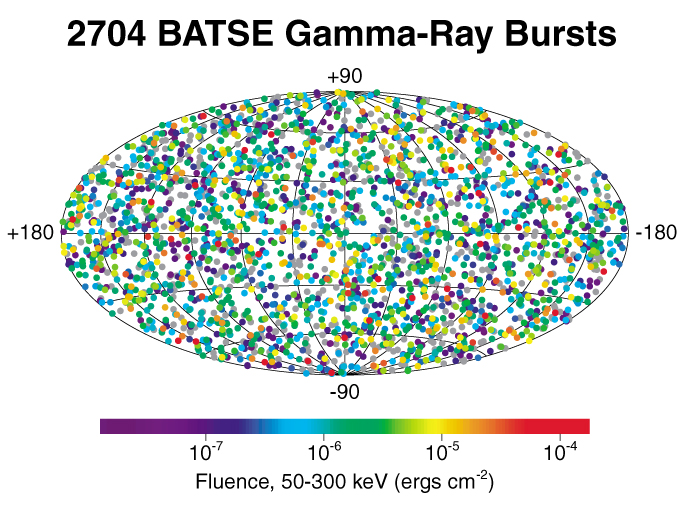
\includegraphics{GRB-BATSE-2704.jpg}
\caption{BATSE 的 GRB 结果。可见这些爆发在宇宙中是各向同性的。图片来源 \href{https://commons.wikimedia.org/wiki/File:BATSE\_2704.jpg}{File:BATSE 2704.jpg on Wikipedia} 。}\end{figure}

现在的理论暗示了某些类型的 GRB 可能跟 core collapse 过程有关,或许与 core collapse 超新星爆发有关。而我们也确实观测到了这样的例子:GRB 980425,红移为 $z = 0.0085$,同样的方向发现的超新星爆发是 1998 bw,为 Type Ic 型。
\end{notice}


\subsubsection{GRB 作为星际战争中的武器}
\label{physics:grb}
由于能量之巨大,我们可以将 GRB(伽玛暴)跟宇宙战争联系起来。然而 GRB 是各向同性的,也就是说在各个方向的 GRB 的数密度大致相同,倘若这是战争,那么就说明战争在我们周围均匀的发生着,然而这是非常难以理解的。因为 GRB 能量之巨大,用来杀害确实是效率之高,但是为了防止射线伤害到自己,需要让射线有一定的方向性。

\begin{notice}{note}{GRB 方向性}

而实际上我们的天体物理理论中,也是考虑 GRB 可能是带有方向性的,因为它的能量太大了,超过了超新星的所有能释放的能量,这是极难理解的。所以理论的解释是,GRB 是由高速运动的物质的 relativistic beaming effect 产生的,这种 beaming effect 可以是的能量的释放集中在物质前进的方向,而且会产生蓝移使得辐射光子的能量变高。这样正好符合 GRB 的要求:集中在某个方向释放能量,不用担心整体的能量太高(太高的话甚至超过超新星的话我们就要担心能量来源了),而且是在高能光子波段。
\end{notice}

设想这样一个场景,帝国 A 与帝国 B 发生了星际战争,帝国 A 为了消灭帝国 B 在一个星系中的据点,便朝向那个方向发射 GRB,高能射线杀死对方绝大多数有生力量。不巧这个 GRB 的方向对准了地球,就被我们看到了。倘若战争这种事情发生非常频繁的话,在整个宇宙尺度上,从地球看来各项同性也就不是那么难以理解了。

\begin{notice}{note}{极端古老的智慧生命}

在 \emph{The highest redshift gamma-ray bursts} 一文中,可以发现有些 GRB 可以发生在非常古老的宇宙中,GRB 最古老的可以接近红移 10。\footnote{
\href{http://arxiv.org/abs/1307.6156}{The highest redshift gamma-ray bursts} - Tanvir, N.R. arXiv:1307.6156 {[}astro-ph.CO{]}
}

那个时候产生智慧生命还要爆发战争是难以理解的。而且即使产生了,他们也要发展出跟当前相同的武器,也是难以理解的。除非,古老的文明一直延续到今天,或者虽然灭亡了但是遗迹被后来的文明发现,复制出了这种武器。

而或许,这种武器就是让恒星坍缩而已,是很容易想到的一种威力巨大的武器。
\end{notice}


\subsubsection{GRB 作为星际飞船推进器的残留}
\label{physics:id13}
星际航行需要消耗的能量非常多,然而更加重要的是,快速的星际航行所需要的能量密度也非常大,这样的过程几乎全部都有光子辐射,如果能量密度很大,产生的会是伽玛光子。例如采用正反物质湮灭作为能源的话,要产生大量的伽马射线,而为了飞船的安全,必然要把这些有害射线导向远离飞船驾驶员的方向,而如果这个方向正好是地球的方向,那么我们就看到了。

如果要解释为外星飞船的话,Mia Molvray 在 1994 年写的这篇 \href{http://www.molvray.com/sf/grb/grblog2.htm}{Gamma Ray Bursters: Unexplained Lights in the Sky} 无疑提供了一些思路。

Mia Molvray 提到了,倘若要往一些遥远的殖民地运动物资,可以使用高速飞行的无人飞船(这样的话也无人在乎狭义相对论的时间效应,因为是无人的)。不管他们使用的是什么能源,不同的发动机有不同的特征,包括 gamma 射线能量随着时间变化的曲线、能量谱等等,会有些许差异。我们或许能够将这些飞船从其他的 GRB 中区分出来。

\begin{notice}{note}{关于 GRB 来自星际飞船的疑问}

然而如果这些 GRB 中真的有些是外星飞船产生的,那么有几个问题难以解释。
\begin{enumerate}
\item {} 
如果是飞船,很可能有船坞,也就是说飞船可能会从相同的地方发射。这与我们会看到同一地点出现多次 GRB,这是没有被观测到的。{[}citation needed{]} 或许解释是,由于 GRB 的方向性,恰巧对准地球只是一个巧合,由于船坞在轨道上,会转动、移动,大多时候不会朝向地球。

\item {} 
GRB 是漫天都是的,而且均匀分布。这个无法解释。唯一可以安慰的就是,飞船产生的只是其中非常非常少的一部分,另一些可能是自然的,可能是战争的,可能是其他的。

\item {} 
为什么是一个爆发,而不是持续的?这个可能的解释的或许飞船并不是完全由这种引擎推动的,或许这种引擎只是用来引发某种效应。例如可能飞船需要点燃引擎几秒钟,然后可以进入超空间了。所以我们只能观测到非常短暂的 GRB。

\item {} 
为什么他们不来找我们地球?这就归结到费米悖论了。不过或许,像《基地》里面的银河帝国一样,这些文明来自地球,但是由于种种原因,他们已经忘却了地球,不想回到地球,被某些谣言所恐吓,想要保存地球这种新生的文明等等。

\end{enumerate}
\end{notice}


\subsection{\index{外星生命和外星文明}外星生命和外星文明}
\label{physics:id14}

\subsubsection{\index{费米悖论}费米悖论}
\label{physics:id15}
\begin{notice}{note}{相关故事}
\begin{enumerate}
\item {} 
黑暗森林出现在了刘慈欣的《三体》系列中。

\item {} 
电影《黑衣人》系列虽然略带搞笑风格,但是也是一种潜在的可能的解释:外星人就在我们身边,但是我们不知道。

\item {} 
电影《2001太空漫游》的说法是外星智慧跟我们想象的形式完全不同。

\end{enumerate}

以上是经典作品。
\begin{enumerate}
\item {} 
拙作 \href{http://multiverse.lamost.org/blog/6455}{《梦与新世界》} 是尝试使用在银河系的旋臂外缘的文明相隔太远,谁也没法飞到对方星系这样的设定。但是这是一个费米悖论局域的解释,也就是说,这个或许只是对于我们太阳系有效,如果靠近银河系银心,恒星数密度更大了,或许大家相距更近些。

\item {} 
关于使用上面的理论来解释费米悖论应用到近未来科幻的一些想法:\href{http://www.guokr.com/blog/793766/}{我们将看到的地外文明} 。

\end{enumerate}

这里部分参考了 \href{http://www.guokr.com/article/283356/}{《科幻概念解读:费米悖论》} 这篇文章。
\end{notice}

\begin{notice}{note}{说明}

关于费米悖论,星际移民中心的 \href{http://interimm.org/exoplanets}{《系外行星文档》} 描述过多种不同的解释。以下为摘录。

\textbf{为了做更多的讨论,我们提出推广的费米悖论:宇宙如此之大,如果一个文明没有发现外星文明,他们或许会问为什么。这样推广之后就不再是基于地球人了,因为这个问题的具体的解释可能跟一个行星的地理位置等有关。}
\end{notice}

我们发现了这么多的行星,可是为什么我们还没有遇到外星人呢?他们都到哪里去了?

1950年,费米问出这个问题(Whre are they?)的时候,我们并没有观测到太阳系之外的行星,在那样一个年代,这样的问题似乎并不是那么有趣。

现在我们已经确认了一千多颗系外行星,几千颗候选,而且这些数字还在继续增长。时至今日,费米的这个问题越来越重要,如果有那么多的栖居地,大家都在哪里呢?

\begin{notice}{note}{费米悖论}
\begin{quote}

宇宙显著的尺度和年龄意味着高等地外文明应该存在。

The apparent size and age of the universe suggest that many technologically advanced extraterrestrial civilizations ought to exist.

但是,这个假设得不到充分的证据支持。

However, this hypothesis seems inconsistent with the lack of observational evidence to support it.

\begin{flushright}
---\href{http://zh.wikipedia.org/wiki/\%E8\%B4\%B9\%E7\%B1\%B3\%E6\%82\%96\%E8\%AE\%BA}{费米悖论\textbar{}维基百科}
\end{flushright}
\end{quote}
\end{notice}

\index{Great Silence}

\paragraph{David Brin 的 Great Silence}
\label{physics:david-brin-great-silence}\label{physics:index-8}
Glen David Brin 在 1983 年曾经发表过一篇名为 \href{http://www.brin-l.com/downloads/silence.pdf}{The Great Silence - the Controversy Concerning Extraterrestrial Intelligent Life} 的论文。在篇论文中,David Brin 导出了一个类似用来描述在当前人类接触到 ETIS,即 Extraterrestrial Intelligent Species,的几率。

\begin{notice}{note}{Drake 方程}

Drake 方程是用来计算(描述)一个完整范围内(例如一个星系)存在可以被探测到的智慧文明的地点(例如行星)的数目:
\begin{gather}
\begin{split}E = R f_g n_e f_1 f_i f_c L,\end{split}\notag\\\begin{split}\end{split}\notag
\end{gather}
其中各个参数的意思在下面的列表中指明。
\begin{itemize}
\item {} 
$R$,该完整范围内的恒星的产生率;

\item {} 
$f_g$,有行星的稳定的(矮)恒星;

\item {} 
$n_e$,每个恒星系中的潜在的可以利用的行星;

\item {} 
$f_1$,上面提到的行星中能产生生命的比率;

\item {} 
$f_i$,所有产生的生命中,演化出智能的比率;

\item {} 
$f_c$,上面提到的智慧生命中制造出可以被检测到的技术的比率;

\item {} 
$L$,带有这样的技术的种类的寿命。

\end{itemize}
\end{notice}

当前(电磁波通信,低速飞船这样的技术水平)人类遇到外星智慧生命的概率(更严格的说是 likelihood)可以用下式计算,
\begin{gather}
\begin{split}C = \frac{1}{N^*}\sum_{j=1}^{E} A_j (n_j+1).\end{split}\notag\\\begin{split}\end{split}\notag
\end{gather}
公式中的 $E$ 就是 Drake 方程计算出来的存在可以探测到的智慧文明的栖居点。$A_j$ 是第 j 种演化出来的智慧生命栖居的或者排出的机器人(例如 von Neuman robot)所占据的栖居点的数目,之所以有个 $+1$ 是因为我们假定这个种类的生命是在其母星上演化出来的,所以他们总共在 $n_j+1$ 个行星上留下了痕迹。$A_j$ 是这类智慧生命的“接触截面”(contact cross-section),是这类生命跟其他的生命有接触的可能性的一个参数。$N^*$ 是“归一化”系数,这里选用有效的恒星数目,去掉了那些不合适的恒星(例如短寿命的恒星,太过靠近的双星等等)。

David Brin 提出了 $n_j$ 的一个形式,
\begin{gather}
\begin{split}n_j = B f_g n_e 4 \pi \int_0^{R_j} e^{-(R_j-r)/v L'}\mathrm d r,\end{split}\notag\\\begin{split}\end{split}\notag
\end{gather}
$B$ 是恒星的数密度,$R_j$ 是该种类的生命的扩展范围的半径,$v$ 是他们的扩展速度(与他们的飞船的速度、繁殖速度等有关),$L'$ 是每个栖居点上面的寿命(与 $L$ 有关)。

这样总结下来,我们关心的量 C,即当前人类遇到外星智慧生命的 likelihood 与这些的参数相关:$f_g$、$n_e$、$f_1$、$f_c$、$f_i$、$L$、$A$. 要解决这个问题,就要分别讨论这些量。

\begin{notice}{note}{关于为什么我们接触不到外星智慧生命}

有很多关于这个问题的讨论。下面从 David Brin 的论文中节选一些列举出来。
\begin{enumerate}
\item {} 
外星智慧生命可能故意躲开我们这样的低级的智能或技术。毕竟相遇之后我们大多在获取新的信息,而不能提供给他们新的信息。

\item {} 
由于电磁波很容易被检测到,所以智慧生命可能会使用 \href{https://en.wikipedia.org/wiki/Bracewell\_probe}{Bracewell probe} 来传递信息,从而减少电磁波的使用和泄露,而且他们也会很注意少使用用来扩展殖民地的机器人(可能会叛变失去控制)。

\item {} 
因为我们的探测方式不对。

\item {} 
外星智慧生命故意隔离我们。可能的原因例如,把我们太阳系当作一个大型的野生动物园来看待(Ball, John A., 1973. Icarus, 19, 347),想要让地球独立发展以期待新的类型的事物出现(Kuiper, T.B.H. \& Morris, M., 1977. Science, 196, 616)。也可能是等待地球上的社会发展成熟,或者觉得地球上人类太过危险(获得与社会发展以及人类心智不相匹配的科技之后)。

\item {} 
Macrolife:摒弃了在行星上生活的方式。例如建造大型飞船游走在太空中,甚至拆解行星作为自己的飞船的原料。例如小说 Macrolife.

\item {} 
某些种类可能害怕太空,在行星上极力发展其他的技术并达到了出神入化的程度,但是依然没有离开自己的行星。例如虽然有过一个短暂的扩展时期,但是很快就蜗居在自己的母星上不出门了。

\item {} 
地球并不是他们想要的地方或者地球无法接近。例如这些智慧生命依靠某种类似虫洞的技术来快速穿越在不同的地方,但是由于某些原因,这类技术不能在地球附近建造,从而与地球没有接触。

\end{enumerate}
\end{notice}

\begin{notice}{note}{小知识:星系围绕银河系中心的公转}

由于公转的角速度不一样,所以径向方向的邻居会变化。
\end{notice}

\index{黑暗森林}

\paragraph{刘慈欣的黑暗森林}
\label{physics:id21}\label{physics:index-9}

\paragraph{\index{Randall Munroe (xkcd) 的 Fish}Randall Munroe (xkcd) 的 Fish}
\label{physics:randall-munroe-xkcd-fish}\begin{figure}[htbp]
\centering
\capstart
\caption{Randall Munroe 的 \href{http://xkcd.com/1377/}{1377号} 漫画。}\end{figure}

\index{智慧扩张模型}

\paragraph{Bezsudnov 和 Snarskii 的智慧扩张模型}
\label{physics:bezsudnov-snarskii}\label{physics:index-11}
他们的论文在这里:\href{http://arxiv.org/abs/1007.2774}{Where is everybody? -- Wait a moment ... New approach to the Fermi paradox} .

果壳网有一篇相关的科普文:\href{http://www.guokr.com/article/129942/}{为什么我们还没遇到外星人?} 。


\section{天体物理}
\label{astro::doc}\label{astro:id1}
天体物理是一门非常非常有趣的学科,因为在这里大家会讨论多种多样的神奇的世界结构。


\subsection{星系系统}
\label{astro:id2}
智慧生命所生活的星系的构成,很大程度上影响了他们的文明的发展方向。就像黄仁宇在书中常常说的地理影响了历史的发展一样,星系的构成,从某种程度上说是一种更加宏大的“地理”(或者“天理”,==!)。而这种星系组成所造成的影响,很可能会比仅仅地面上的那些地理要重大的多。

\begin{notice}{note}{科学问题}

当然,从科学上讲,如果我们要设置一颗行星在一个恒星系统中,那么我们需要注意很多问题,例如,一个太过复杂混乱的恒星系统,例如三体系统,可以产生行星么?产生行星的概率多大?或者,我们可以设定为行星不是在该恒星系统产生的,而是在其他地方产生,由于某些变故,才被注入到这个系统中来。变故的可能比如星系大冲撞等等外来的强大的引力的干扰。
\end{notice}


\subsubsection{处在宿主恒星不同阶段的系统}
\label{astro:id3}
比较有趣的是处在红巨星时期的情况,以及处在中子星或者白矮星时期的行星的发展情况。

这部分是大众比较熟悉的,所以就不再仔细讨论了。


\subsubsection{带有周期性灾难爆发的行星系统}
\label{astro:id4}
行星如果围绕着一个带有吸积盘的系统旋转,例如行星围绕由中子星和恒星组成的系统旋转(或者非常靠近这样一个系统),而中子星形成吸积盘,除了吸积盘的轫致辐射和黑体辐射的叠加,还可能有类似核闪耀的事件。

\begin{notice}{note}{补充知识}

恒星如填充了 Roche lobe,那么恒星的物质就会被中子星夺走,并且形成吸积盘。而在一个带有强磁场的中子星周围,吸积盘的物质并不会直接落在中子星表面的任何地方,而是落入两端磁极。原因是磁场对于等离子体的强力的束缚作用。然后由于落入两极的物质会形成 shockwave,在 shockwave 发生的时候,可能会发生核反应,从而释放更多的能量。取决于不同的情况,这样的过程可能会周期性的发生。
\end{notice}

那么在这样一个行星系统中的生命,就会周期性的遇到一些大的爆发。
\begin{enumerate}
\item {} 
如果爆发强度太大,那么会导致几乎所有生命完全灭绝。

\item {} 
如果强度不是那么大,会杀死部分生命,导致周期性的物种大灾难。

\item {} 
不是很强的时候,会有很强的高能射线导致变异突增。

\end{enumerate}

这样就会有不同的情况可以讨论,也就导致了不同的文明的发展。


\subsubsection{处在星系盘面上方的行星系统}
\label{astro:id5}
由于某些外力的原因,一个行星系统可能会被抛到星系盘面的上方。这样一来,该行星上看到的银河系,就不在是一条银河,而是一个银盘,他们的天文观测,也会因为庞大的圆盘的遮挡,受到干扰。

设想一下,那将是一个多么壮观的场景,夜晚来临,头上有个发光的圆盘,而且中间明亮,四周暗弱。


\subsection{天体级别的推进技术}
\label{astro:id6}

\section{交叉学科}
\label{interdispline::doc}\label{interdispline:id1}
交叉学科的发展,常常给我们带来意想不到的收获。在科幻中,交叉学科也会是科幻点子里面非常出彩的部分。


\subsection{生物体增强}
\label{interdispline:id2}
\index{精神感应}

\subsubsection{精神交流}
\label{interdispline:index-0}\label{interdispline:id3}
\begin{notice}{note}{待相关专业验证}

目前这只是点子,尚需相关专业的人员验证。
\end{notice}

首先我们搞清楚如何将人的思维转换成电磁波。

然后我们需要制作出仅仅由生物体可以合成的物质来组成的电磁波发射接收调制解调等等一系列用来通信的工具。这样可以植入人体,但是这显然不够,我们希望这些部件自己生长出来。

我们找到对应的基因组成,在合适的位置嵌入人体受精卵或者直接嵌入到卵细胞线粒体(这样就可以通过母亲进行遗传了)。这样无需进行手术,新生儿就会有相应的部件将部分思维转换成电磁波发送给其他人,其他人接受到之后可以直接在大脑中阅读这些思维。并且,这是可以遗传给下一代的。

\begin{notice}{note}{相关故事}

\href{http://multiverse.lamost.org/blog/6433}{火星的天空} 就是用了这样一个想法。
\end{notice}


\section{科幻中的社会元素}
\label{social::doc}\label{social:id1}
这章不仅仅包括社会科幻,还包括科幻中的社会元素。讲故事几乎必然会用到社会元素,在相应的大背景下合情合理的有新意的社会元素对于故事也是非常重要的。


\section{历史}
\label{history::doc}\label{history:id1}
人类对历史的记录非常不完善,因此历史上有很多谜团或者说可以被利用的“漏洞”。


\subsection{新的考古发现}
\label{history:id2}
我们可以安排很多新的历史和考古发现,通过这些“新的发现”来提供重新解释历史或者发展未来。


\subsubsection{解码古时候的声音记录}
\label{history:id3}
\begin{notice}{note}{Note:}
这只是一个插入新的考古发现的例子。
\end{notice}

人类能够留下图像记录,因为相比之下,图像更容易重现出来。而声音的重现却困难的多。倘若我们想要在背景中插入什么重要的线索。

例如,可以非常久远的雕刻实际上是声音文件,可以解码,播放出来。这样我们可以解密那个时代的口语。甚至如果剧情需要,可以通过那个人指出一个天大的秘密,这也是很多故事热衷的情节。

至于如何解码声音记录,如果没有校准文件,只能通过运气或者暴力破解。实际上我们可以讲雕刻的记录图像化,然后通过计算机暴力破解。

再举一个例子。这次我们可以拿 Leonardo da Vinci 开刀。

这位天才实际上发明了记录声音的方法,虽然他没能还原记录的声音,但是他确实将许多重要的声音记录下来了。然后我们将来发现了这些声音记录并且解码出来。

另一个思路是我们可以假设他发明了记录声音的方法,并且能够解码,用于一些秘密通信只用,这也是为什么我们看不到历史中记载他的发明。这样我们可以重新解释文艺复兴的历史,写出一段精彩的故事。


\section{超能力}
\label{superpower::doc}\label{superpower:id1}
本章节讨论在科幻、玄幻、魔幻等等作品中出现的超能力,配合恰当的科学解释,我们可以对超能力进行二次开发或者扩展。

\begin{notice}{note}{Todo}

需要写的超能力人物列表
\begin{itemize}
\item {} 
万磁王

\item {} 
炮姐

\item {} 
黑子 Kuroko Shirai

\item {} 
暴风女

\end{itemize}
\end{notice}


\subsection{远程控制物体}
\label{superpower:id2}

\subsubsection{万磁王(Magneto)}
\label{superpower:magneto}
\begin{notice}{note}{万磁王的设定}

万磁王可以控制金属物体,并且可以使得金属物体变形(从电影的特效来看,类似熔化之后的那种变形)。

在万磁王起源的片段中,巨大的铁门居然被掰弯,以及在后面的从塑料牢笼逃跑的情节中,万磁王利用从食物中获得的金属在空中飞行。
\end{notice}

从万磁王的名字(Magneto)是跟磁有关的,因此直观的理解,万磁王通过磁场(或者说控制金属的磁性)来控制物体。考虑到电影中那种变形看似熔化,再加上控制金属物体,所以万磁王的能力很可能对于金属特有的晶格结构有关。

实际上想要远距离抓住金属,显然也应该还是电磁力的范畴(因为引力和弱相互作用太弱,而强相互作用作用距离太短)。而晶态金属特有的,能带结构算是比较重要的,因为这决定了金属的高电导率和热导率,也决定了磁性。

\begin{notice}{note}{金属、能带与磁性}

在单个的原子中,或者说在单个的球对称的势井中,我们可以计算(估算)电子的行为,结果是电子形成分立的轨道,对应不同的能级。然而金属的晶格结构中,有些电子是金属晶格共有的,也就是说,势函数变得复杂,但是却还有周期性,这使得电子的部分分离的能级之间的能量差异变得很小,而考虑到不确定性原理,这些细小的能级几乎是连续的。因此大家成为**能带**。

电子会优先填充低能的能级,在基态电子聚集在一些低能的能带上,这些叫做**价电子**,对应的能带叫做**价带**。而有些能带尚未被电子占满,这些能带上的电子可以自由的移动,从而导电或者导热。这样的能带叫做**导带**。

金属中磁性的起源是电子的自旋,因此能带上自旋向上和向下的电子的数目的差异决定了金属的磁化。
\end{notice}

考虑到要抓住物体包括举起物体,万磁王需要控制物体的抗磁性和顺磁性或者铁磁性。而控制这些,最直接的方法就是可以控制电子的自旋。

因此,万磁王可以**将一定数目的自旋翻转**。而且必须是有控制的主动翻转,不然他自己就必须一直永远带极强的磁性。\textbf{这解释了万磁王可以控制金属物体。}

然而,这会遇到一个问题,在 \href{http://www.douban.com/people/emptymalei/status/1535791054/}{豆瓣我说} 与 \href{http://www.douban.com/people/Raman/}{大使} 的讨论中,涉及到了如何防止在万磁王施法的时候,不小心被附近的金属刀叉插死(施法的时候要产生磁性才能控制物体嘛,附近有刀叉就飞过来,插死自己了)。大使提到可以通过改变周围的磁导率形成一个屏蔽。

具体说来如果要屏蔽周围磁场,其中的两种方法分别是形成高磁导率的区域是的磁场主要影响自己想要影响的区域,或者在周围的铁磁性物体周围形成高磁导率区域从而对这些物体屏蔽磁场。而控制磁导率,最好是能够产生许多磁偶极子。而万磁王大多时候所能利用的只是空气,所以只能借助空气,在一个区域产生足够多的磁偶极子。


\section{架空历史}
\label{alternatehistory::doc}\label{alternatehistory:id1}
架空历史故事最常见手法是从人类历史上某个事件开始给出一条完全不同的路径,一个非常出色的典范就是《差分机》——假定十九世纪的差分机并没有失败而是快速的发展起来人类的历史会是如何。

若模仿差分机模式,我们需要找出历史上可能的分叉点,看到历史的一条迥然不同的路径。


\subsection{路径积分历史学}
\label{alternatehistory:id2}
在我们列举具体的架空历史的方案之前,先看一下历史学。

此时此刻,我所想到的是,倘若我们物理学中路径积分的想法应用到历史中呢?

\begin{notice}{note}{心理史学}

在《基地》系列中,Seldon 的心理史学,有一部分非常有可能使用路径积分的方法来实现。

创建第二银河帝国,Seldon 要考虑的是未来可能的路径,以及一个自己想要的未来状态(某种状态的第二帝国,为避免剧透,暂不透露细节)。也就是说,Seldon 知道初始状态以及结束的状态。
\end{notice}

既然《基地》系列中, Seldon (或者第二基地)知道初末状态,那么仿照 QFT 或者统计物理或者经济物理里面的路径积分方法,如果知道作用量,就可以得知不同路径的相对概率。然后就可以给出一条 \textbf{正则路径} 。
\begin{figure}[htbp]
\centering
\capstart

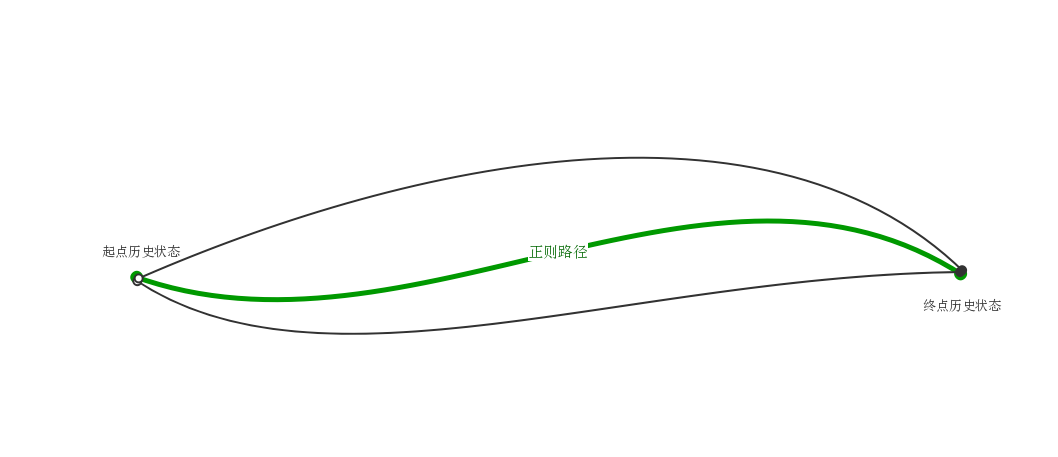
\includegraphics{psychohistory-canonical.png}
\caption{从历史的一个点到另一个点有很多可能的路径,中间的加粗为最直接的路径。这里我们的理论定义了最直接,最好是使最小作用量原理成立。各条路径的相对概率是可以给出来的。}\end{figure}

《基地》故事中,第二基地可以说出某些事情发生的概率,以及采取某些措施之后有多大的概率回到某个状态。

如前所述,我们知道不同路径的概率,然后我们对所有的经过这个事件的所有的路径求和(积分),我们就可以得到这个事件发生的概率(其实是个相对概率)。
\begin{figure}[htbp]
\centering
\capstart

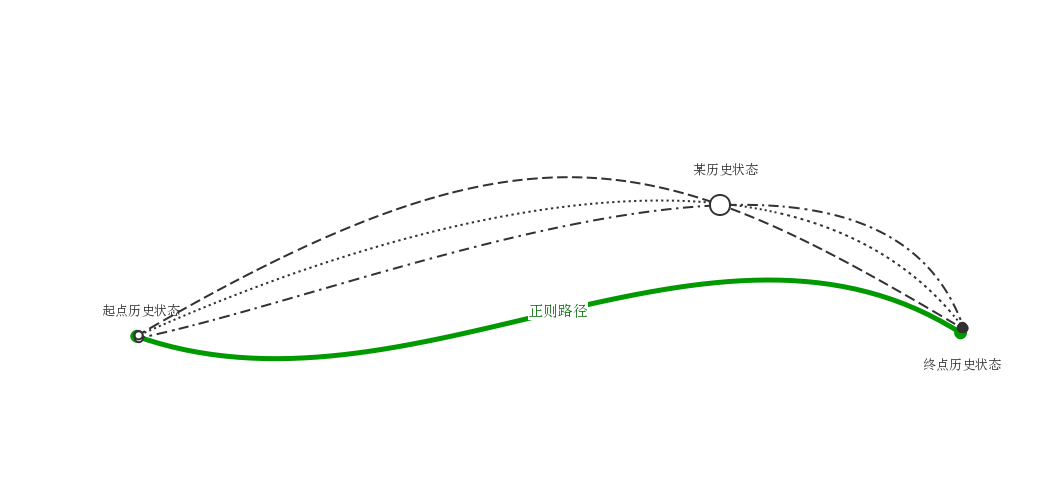
\includegraphics{psychohistory-prob.png}
\caption{将所有的经过“某历史状态”的可能路径概率求和(或积分),就可以得到该状态发生的相对概率。}\end{figure}

然后我们以此状态(“某历史状态”)为起点,修改作用量(添加额外的影响,也就是自己想要采取的措施),计算当前这个已经偏离正则路径在点,回到正则路径上的所有的可能点的可能路径(这是一条从偏离点回到原来设定的正则路径的新的正则路径)。然后对所有的这些求和(或积分),就可以给出采取了这个措施之后,回到原始正则路径的相对概率。
\begin{figure}[htbp]
\centering
\capstart

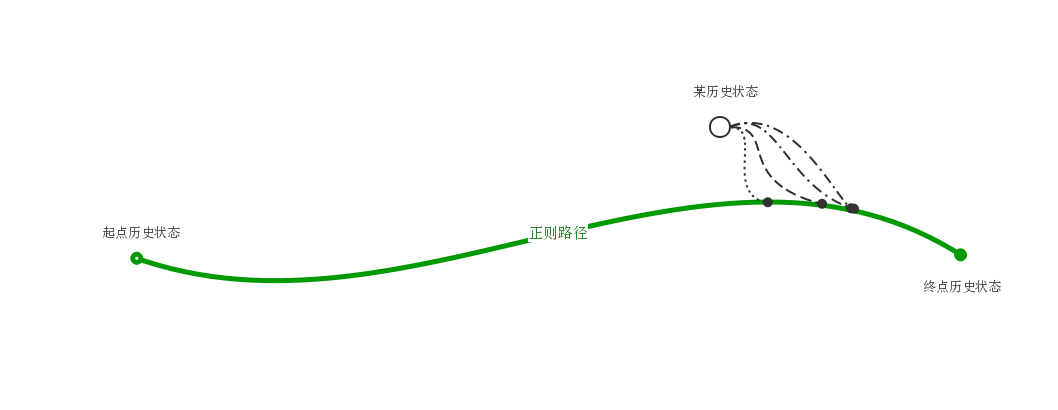
\includegraphics{psychohistory-modi.png}
\caption{如果要从“某历史状态”回到一开始的正则路径上,我们需要以“某历史状态”为起点,计算所有可能的回归到一开始路径的所有的可能路径,并且可以给出概率。如果这个概率偏低,就需要对原来的作用量施加影响加以改变,使得新的作用量下面,回归一开始的正则路径的相对概率提高。}\end{figure}

然而,不必拘泥于小说故事,我们不必回到原始的正则路径。我们需要做的,只是达到我们的目的——第二银河帝国,所以我们只需要计算采取某种某种措施之后,新的正则路径是什么。
\begin{figure}[htbp]
\centering
\capstart

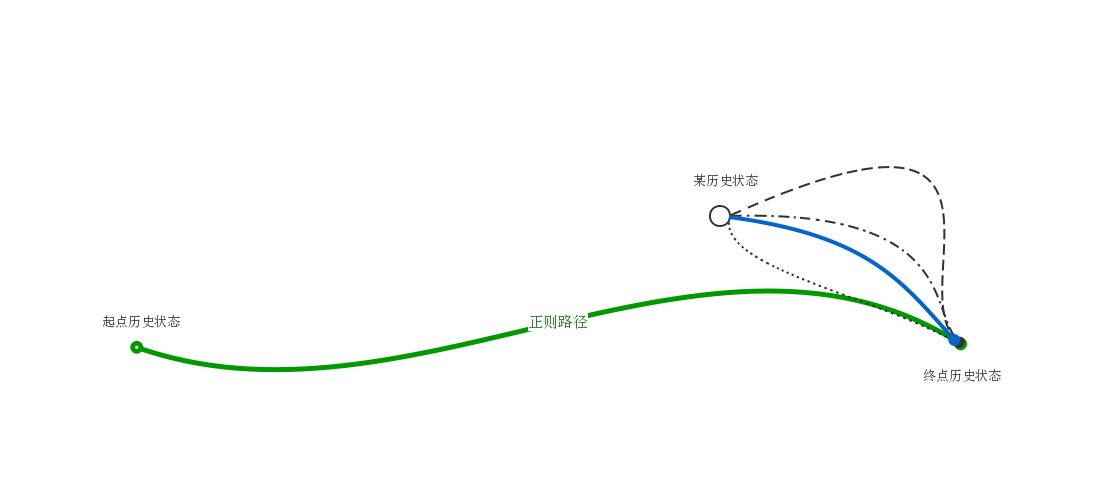
\includegraphics{psychohistory-modi2.png}
\caption{实际上并不需要拘泥与《基地》故事,非要回归原来的路径。最一般的做法是通过修改作用量,增加到达目的地的概率。}\end{figure}

\begin{notice}{note}{历史的终点是什么}

可是,我们如何知道历史到达上面所有提到的终点状态的绝对概率呢?倘若我们有一个历史的必经之点,那么我们就可以以此点为参照,计算出经过我们想要的点的概率。然而这是非常困难的。
\end{notice}


\chapter{参考及备注}
\label{index:id3}
本文档由 \href{http://interimm.github.io/}{星际移民中心} 提供支持。

文档内容若无特殊说明使用 CC BY-SA 协议。



\renewcommand{\indexname}{Index}
\printindex
\end{document}
